\chapter{Main Server configuration}
\label{chapter:server}

In order to control the current features already developed and used in the car it is used a \href{https://www.raspberrypi.org/products/}{Raspberry PI} (currently version 3 model B). The \acrlong{Rpi}, from now on denoted as \acrshort{Rpi}, is a \gls{SBC} affordable and low power, widely used among community and developed by Raspberry Pi Foundation. Figure \ref{fig:raspberrypi_pinout} show the relevant parts of \gls{Rpi} and also the pinout labels.

\begin{figure}[!h]
	\centering
	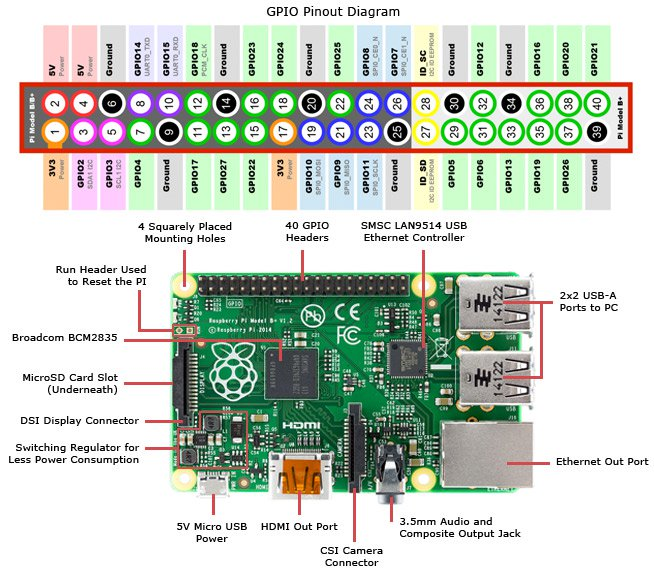
\includegraphics[width=0.9\linewidth]{figures/raspberry_pi_circuit_note_fig2}
	\caption[Pinout labels for RaspberryPi 3]{Pinout labels for RaspberryPi 3 (\href{https://www.jameco.com/Jameco/workshop/circuitnotes/raspberry-pi-circuit-note.html}{source})}
	\label{fig:raspberrypi_pinout}
\end{figure}

\section{Requirements}
For using the \gls{SBC} it is required the following hardware:
\begin{itemize}
	\tightlist
	\item \textbf{Raspberry Pi \gls{SBC}} Recommended version at least 3 since it has a built in wifi.
	\item \textbf{MicroSD card} Recommended with 8Gb capacity at least.
	\item \textbf{Power Supply} Recommended 2.5 Amps . While developing, it is used as the main power for the \gls{SBC}.
	\item \textbf{Host computer (any \gls{OS})} with internet and ability to read MicroSD cards.
	\item \textbf{Ethernet cable} for connecting to router/switch for internet access. It can also be used an crossover cable connecting directly to PC if it is able to share internet connection.
\end{itemize}

\section{Initial Preparation}
This preparation will focus on providing instructions to a minimal headless setup. For this reason, the recommended \gls{OS} image version is the Raspbian Lite.

For this step it is recommended to be used the \href{https://etcher.io/}{Etcher} software for burning the \gls{OS} image into microSD card. It is assumed the user is familiar with ssh capable software, for example \href{https://www.putty.org/}{Putty}. 
The next steps are mainly based in the documentation guide provided by \cite{raspberry_install_guide}.

\begin{enumerate}
	\tightlist
	\item Download the \gls{OS} image, Raspbian Lite version in \href{https://www.raspberrypi.org/downloads/raspbian/}{here}
	\item Connect the MicroSD to host computer.
	\item Open Etcher and:
	\begin{enumerate}
		\item Select \gls{OS} image or zip file that have been downloaded.
		\item Select the SD card you wish to write your image to.
		\item Review your selections and click 'Flash!' to begin writing data to the SD card.
		\item after successful write, continue to next step.
	\end{enumerate}
	\item From microSD card, open the boot partition.
	\item Create a new blank file with name "ssh" without extension. This will allow to enable the ssh daemon at first boot time.
	\item Remove card from host computer and insert on raspberry PI.
	\item Plug in the Ethernet cable and connect the \gls{Rpi} to the same  local network as host computer.
	\item Plug in the power supply to \gls{Rpi}.
\end{enumerate}

\begin{figure}
	\centering
	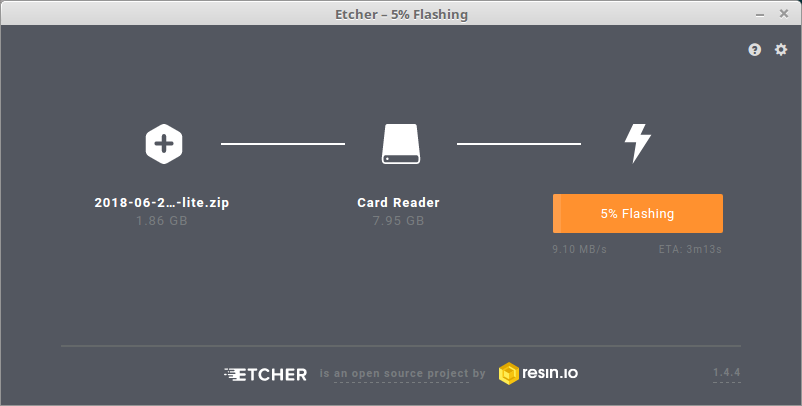
\includegraphics[width=0.5\linewidth]{figures/Etcher_flashing.png}
	\caption{Etcher flashing image to microSD card}
	\label{fig:etcher_flashing}
\end{figure}

If everything went as expected, the \gls{Rpi} will start to boot and prepare the first setup. It will be seen led light blinking indicating activity. After a few minutes, it should be possible to access it remotely via ssh

%-------------------------------------------------------------------------------
% create a remote access setup
%-------------------------------------------------------------------------------

\subsection{Remote access}
The next step is to find the ip address of the \gls{Rpi}. For example, in linux terminal type \console{arp -a}. In figure \ref{arp_example} is seen an output example. In red stroke is shown the \gls{MAC} address of a \gls{Rpi}. Every \gls{MAC} is unique and the first three bytes are fixed in every \gls{Rpi} wich correspond to organizationally unique identifier \cite{mac_wiki} associated to Raspberry Pi Foundation, B8:27:EB \cite{wireshark_mac}.

\begin{figure}[hb]
	\centering
	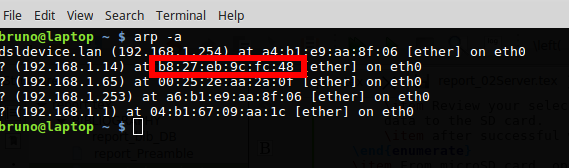
\includegraphics[width=0.7\textwidth]{figures/arp_example}
	\caption{arp -a command example output}
	\label{arp_example}
\end{figure}

Perform the first login with using the default login details as shown in table \ref{tab:default_login}.
Using the discovered ip for the \gls{Rpi}, in Linux, the first login  may be performed using \console{ssh pi@\textless ip-of-Rpi\textgreater} command and entering the default password.

\begin{table}[!h]
	\centering
	\begin{tabular}{rl}
		\toprule
		\textbf{username:}& pi\\
		\textbf{password:}& raspberry\\
		\bottomrule
	\end{tabular}
	\caption{Default login details for \gls{Rpi}}
	\label{tab:default_login}
\end{table}

\begin{figure}[!h]
	\centering
	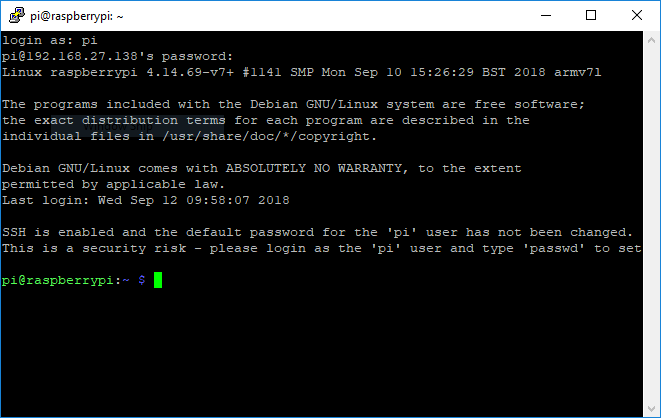
\includegraphics[trim={0 3cm 0 0}, clip, width=0.5\textwidth]{figures/ssh_sucessfull.png}
	\caption{SSH sucessfull login}
	\label{fig:ssh_successfull}
\end{figure}

%-------------------------------------------------------------------------------
%  initial update and configurations 
%-------------------------------------------------------------------------------
\subsection{Initial update and configuration}
If the user as been granted with permission to login, the next steps are used to perform a few tweaks.
To do that user must use the command \console{sudo raspi-config}. Example output is seen in figure \ref{fig:raspi_config}.

\begin{figure}[!hb]
	\centering
	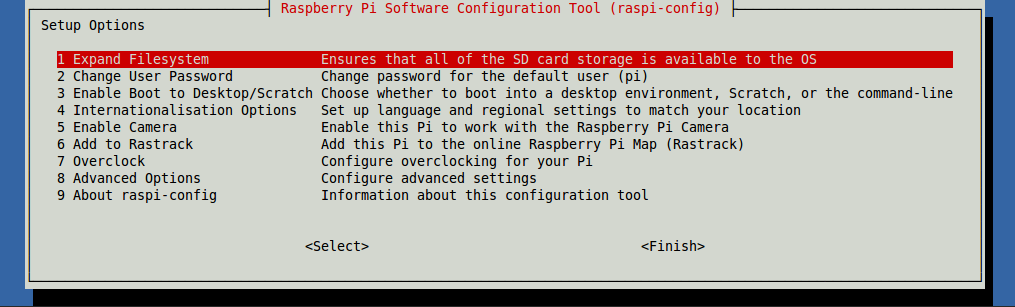
\includegraphics[width=0.7\textwidth]{figures/raspi-config}
	\caption{Raspi-config example output}
	\label{fig:raspi_config}
\end{figure}

It is recommended to configure the following:

\begin{itemize}
	\tightlist
	\item Set Keyboard Layout
	\item Update to lastest software
	\item Set Timezone
	\item Set language [optional]
	\item Change default login password
	\item Configure Wifi-zone [if present]\\
    \begin{mdframed}[backgroundcolor=red!20, roundcorner=10pt, innertopmargin=5pt, innerbottommargin=5pt, skipabove=0pt]
        If you are connected directly to a switch via Ethernet cable, skip wifi configuration.
    \end{mdframed}
	\item Enable \gls{SPI} for \gls{CAN} controller
	\item Enable \gls{I2C} for RTC
	\item Set hostname
	\item change default password
	\item change memory for GPU
\end{itemize}

The current settings are presented in table \ref{tab:suggested_config}. 

\begin{table}[h]
	\centering
	\begin{tabular}{rl}
		\toprule
		\textbf{Username:}& pi\\
		\textbf{Password:}& fiatelettra\\
		\textbf{Hostname:}& raspberrypi\\
		\textbf{wait for network at boot:}& no\\
		\textbf{Language:}& en\_GB.UTF-8 UTF-8\\
	    \textbf{Timezone:}& Europe $\rightarrow$ Lisbon\\
	    \textbf{Keyboard layout:}& pt\_PT\\
	    \textbf{WIFI country:}& PT\_Portugal\\
	    \textbf{SPI:}& on\\	
		\textbf{I2C:}& on\\
		\textbf{Memory split:}& 16 (minimum since is running headless)\\
		\bottomrule
	\end{tabular}
	\caption{Suggested details for \gls{Rpi}}
	\label{tab:suggested_config}
\end{table}

After successfully changed the settings, perform a full update and upgrade by running:
\begin{lstlisting}[frame=none,language=bash,backgroundcolor=\color{gray!15},numbers=none]
sudo apt update && sudo apt upgrade -y
\end{lstlisting}


\section{Prepare CAN interface}
\label{section:can}
The current protoboard uses the \gls{IC} \href{https://www.microchip.com/wwwproducts/en/MCP2515}{MCP2515} as \gls{CAN} network controller and \href{https://www.microchip.com/wwwproducts/en/MCP2551}{MCP2551} as \gls{CAN} transceiver. Figure \ref{fig:proto_can} shows the used protoboard with highlighted connections names and parts.

The schematic circuit implemented in the protoboard is present in figure \ref{fig:schematic_proto_can}.
Current raspbian kernel, automatically support the can interaction via \gls{SPI} to \gls{IC} MCP2515, making it available via SocketCAN. To enable that, it is necessaries to configure MCP2515 driver on device tree overlay and install the can-utils package.
\begin{itemize}
	\tightlist
	\item Install can-utils using \console{sudo apt install can-utils}
	\item Enable MCP2515 overlay by using \console{sudo nano /boot/config.txt} and append at end:
	\begin{lstlisting}[label={lst:boot_settings},frame=none,language=bash,backgroundcolor=\color{gray!15},numbers=none,basicstyle=\ttfamily]
#CAN bus controllers
dtoverlay=mcp2515-can0,oscillator=16000000,interrupt=25
dtoverlay=spi-bcm2835
\end{lstlisting}
	\item To enable the interface at boot time, use \console{sudo nano /etc/network/interfaces} and append at end:
	\begin{minipage}{\linewidth} % to avoid breaking on page
\begin{lstlisting}[frame=none,language=bash,backgroundcolor=\color{gray!15},numbers=none,		basicstyle=\ttfamily]
auto can0
iface can0 inet manual
  pre-up /sbin/ip link set can0 type can bitrate 1000000 \
  triple-sampling on restart-ms 10
  up /sbin/ifconfig can0 up
  down /sbin/ifconfig can0 down
\end{lstlisting}
	\end{minipage}
\end{itemize}
This will enable the \gls{CAN} interface at boot time with the setting present in table \ref{tab:can_settings}.

\begin{figure}[!hb]
	\centering
	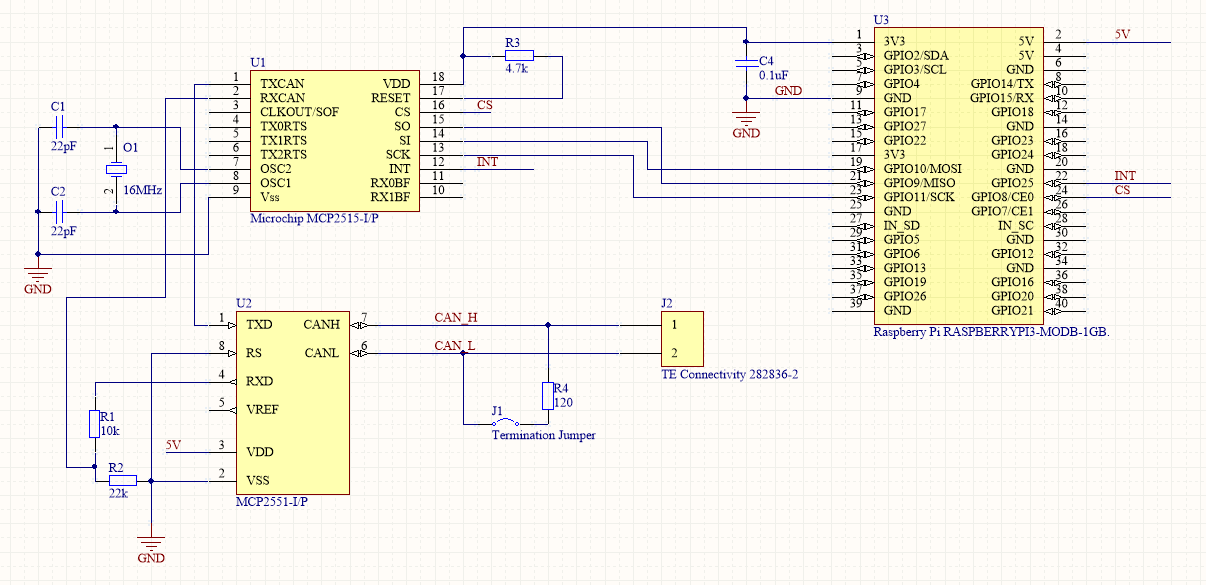
\includegraphics[width=0.9\linewidth]{figures/protoschematic}
	\caption{CAN protoboard schematic}
	\label{fig:schematic_proto_can}
\end{figure}

\begin{figure}[!h]
	\begin{minipage}{0.49\linewidth}
		\centering
		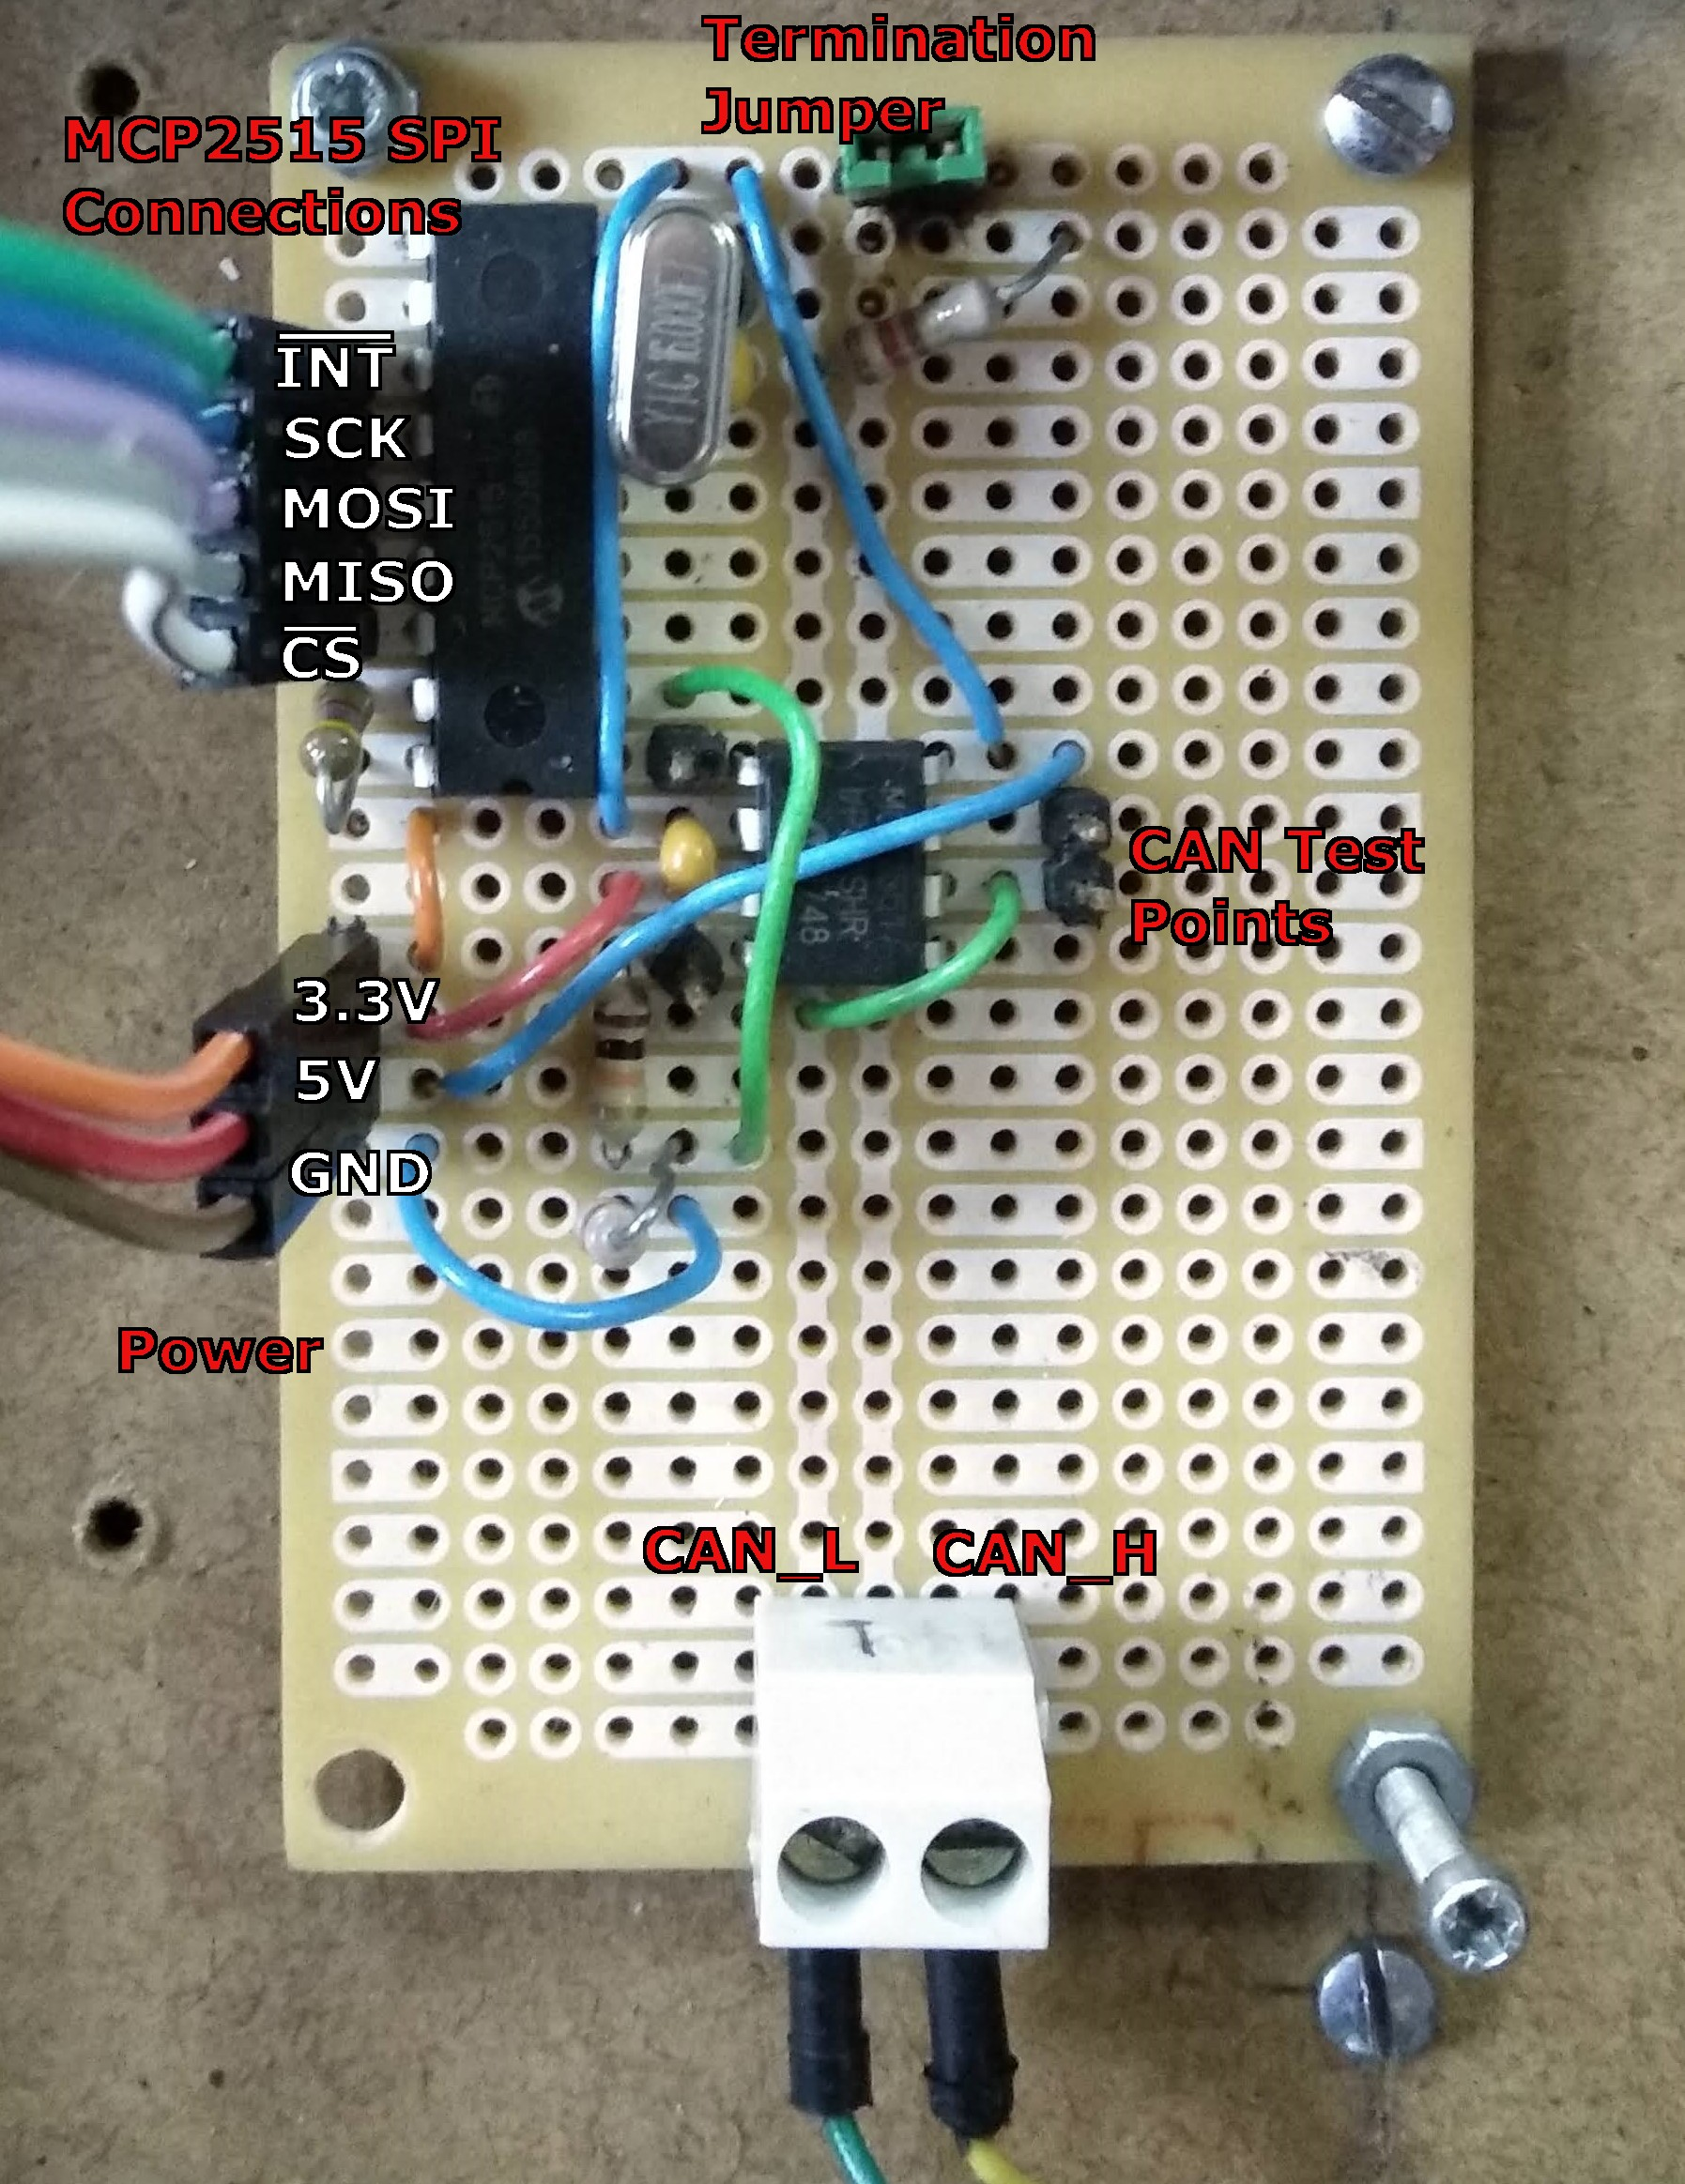
\includegraphics[width=1\linewidth]{figures/proto_can}
		\caption{Protoboard designed for CAN interface}
		\label{fig:proto_can}
	\end{minipage}
	\begin{minipage}{0.49\linewidth}
		\centering
		\begin{tabular}{rl}
			\toprule
			\textbf{Parameter} & \textbf{Value}\\
			\midrule
			Bitrate & 1Mbps\\
			Triple Sampling & on\\
			Sampling point & 0.75\\
			Restart & 10ms\\
			\bottomrule
		\end{tabular}
	    \captionof{table}{CAN used settings}
	    \label{tab:can_settings}
	\end{minipage}
\end{figure}

The protoboard is considered temporary and new board as been designed and projected to include not only a \gls{CAN} controller but also a \gls{RTC} chip, a battery holder for \gls{RTC} chip and a DC-DC converter to power \gls{Rpi} from 12V battery pack. In figure \ref{fig:board_can} is show the proposed and developed circuit for replacing the protoboard. The respective schematic is present in appendix \ref{appendix:can_schematics}. Suggested board was designed in Eagle Software and files are also included in the Github repository.

For connecting the protoboard please refer to figure \ref{fig:raspberrypi_pinout} to see the respective pins in the \gls{Rpi} side.

\begin{figure}[!hb]
	\centering
	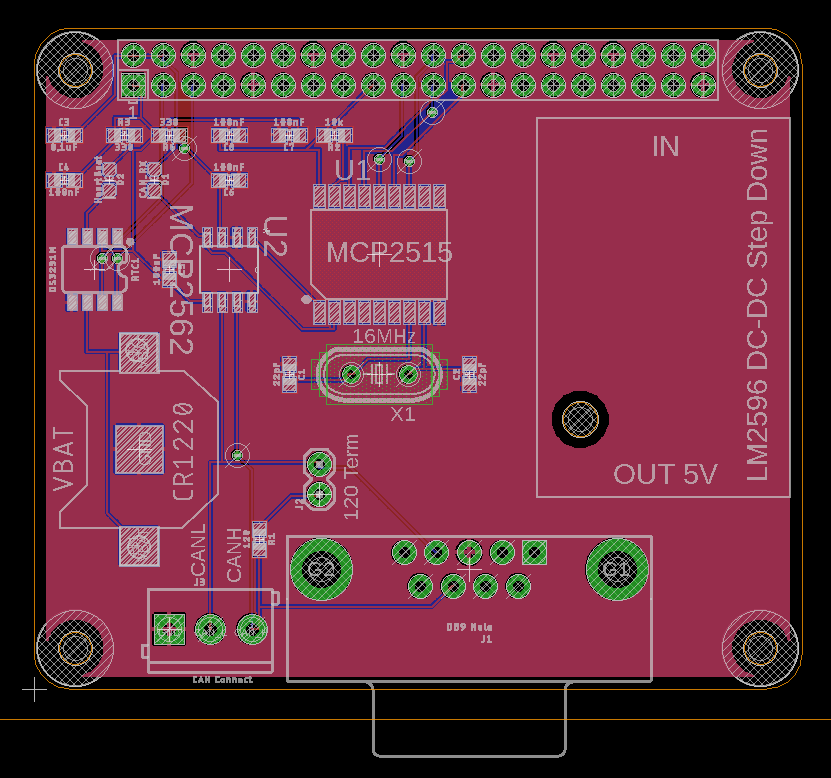
\includegraphics[width=0.6\linewidth]{figures/Viena_Rpi_CAN_interface_board}
	\caption{Proposed CAN interface board for future use}
	\label{fig:board_can}
\end{figure}


%-------------------------------------------------------------------------------
% create a additional packages installation
%-------------------------------------------------------------------------------
\section{Additional packages installation}
The following list describes additional package installation that are currently used or are planned to be used.
\begin{description}[style=nextline]
	\item[python3-pip] Required to enable pip manager.
	\item[python3-venv] To enable the creation of virtual environments.
	\item[libatlas-base-dev] Required to install numpy package.
	\item[mosquitto] Local \gls{MQTT} broker used currently in development branch. It might be useful to install also the \console{mosquitto-clients}.
	\item[build-essential] Required if needed to compile anything.
	\item[git] Add git support to raspbian.
	\item[nginx] Local lightweight web server application used to control or see current status of vehicle (in development) 
	\item[ufw] Firewall interface to improve security.
	\item[dnsmasq] Provides network infrastructure for small networks as \gls{DNS}, \gls{DHCP}. Will be used to configure \gls{Rpi} as an \gls{AP}.
	\item[hostapd] Daemon for configuring and enabling the \gls{AP}
\end{description}

\section{Post-Installation Procedures}
After installing the recommended packages, user should perform several configurations. In this section is described each of them.

\subsection{Adding user to groups}
After adding user to any group, \textbf{a logout must be performed to changes take effect}. Changes can be confirmed by using the command \console{groups} that prints the groups current user is in.
\begin{description}[style=nextline]
	\item[www-data] Grant user ability to perform changes on /var/www. Run \console{sudo adduser pi www-data}
	\item[dialout] Grant user ablility to use ports. Run \console{sudo adduser pi dialout}
\end{description}

%-------------------------------------------------------------------------------
% installing mosquitto
%-------------------------------------------------------------------------------
\subsection{Configuring MQTT Broker}
Current and planned development roadmap use \gls{MQTT} brocker to change messages between user or high level software and hardware interface. It is also used websockets and in this section will be shown how to enable it. The current used broker is \href{https://mosquitto.org/}{mosquitto}. If not already installed, use:\\ \console{sudo apt install mosquitto} \\
After installation edit mosquitto.conf by using \console{sudo nano /etc/mosquitto/mosquitto.conf} and add an additional port for websockets protocol. If advanced configuration is need refer to \cite{mosquitto_conf}. In order to use mosquitto with \gls{QoS} of 1 or 2 and accept large queues, it was increase maximum queued messages to 10000. Also, since it is not required, persistence file was disabled.

\begin{lstlisting}[frame=none,language=bash,backgroundcolor=\color{gray!15},numbers=none,		basicstyle=\ttfamily]
pid_file /var/run/mosquitto.pid
persistence false
persistence_location /var/lib/mosquitto/

log_dest file /var/log/mosquitto/mosquitto.log

include_dir /etc/mosquitto/conf.d

port 1883
listener 8080
protocol websockets

# max_inflight_messages 0
max_queued_messages 10000 
\end{lstlisting}

Since official repository did not have the latest release of mosquitto, it was necessary to
manually update it using:

\begin{lstlisting}[frame=none,language=bash,backgroundcolor=\color{gray!15},numbers=none,		basicstyle=\ttfamily]
wget http://repo.mosquitto.org/debian/mosquitto-repo.gpg.key
sudo apt-key add mosquitto-repo.gpg.key
cd /etc/apt/sources.list.d/
sudo wget http://repo.mosquitto.org/debian/mosquitto-stretch.list
sudo apt update
sudo apt upgrade
\end{lstlisting}

In order to discuss future implementations it was tested the ability of using the \gls{MQTT} interface for fast rate messages. For that, in table \ref{tab:mqtt_results} are shown different approaches using local vs online brokers and implementation on \gls{Rpi} vs local laptop (Lenovo T480).

As summary, test conditions are as follow:
\begin{itemize}
	\tightlist
	\item 1000 messages sent, using an Int32 with the number of message as payload.
	\item Same \gls{QoS} in both ends.
	\item Using same PC to run the sender and receiver clients (Lenovo T480)
	\item Comparison between local MQTT broker (mosquitto), running in RaspberryPI 3 and Laptop, as well as online servers.
	\item Mean of 5 consecutive tests.
	\item Transport used is websockets in both clients.
\end{itemize}

\begin{table}
	\centering
	\begin{tabular}{lccrrrr}
		\toprule
		\multicolumn{7}{c}{\textbf{Receiving Results}}\\
		\textbf{Server} & \textbf{Is local?} & \textbf{QoS} & \textbf{Mean} & \textbf{std} & \textbf{min.} & \textbf{max.}\\
		\toprule
		mosquitto         & Yes     &0    & 9754.14        &1735.97 &7316.35 &11653.73  \\
		mosquitto         & Yes     &1    & 4917.01        &172.89  &4680.69 & 5125.19  \\
		mosquitto         & Yes     &2    & 3663.86        &234.97  &3339.15 & 3999.98  \\
		\midrule
		mosquitto (Rpi)   & Yes     &0    & 820.48         &36.45   &781.01  & 860.08   \\
		mosquitto (Rpi)   & Yes     &1    & 780.07         &73.96   &650.22  & 835.46   \\
		mosquitto (Rpi)   & Yes     &2    & 390.70         &30.80   &356.01  & 426.96   \\
		\midrule
		mosquitto.org     & No      &0    & 103.71         & 4.47   & 96.85  & 108.64   \\
		mosquitto.org     & No      &1    & 107.87         & 9.85   & 90.55  & 113.12   \\
		mosquitto.org     & No      &2    & 57.69          & 0.65   & 56.89  & 58.44    \\
		\midrule
		broker.hivemq.com & No      &0    & 3209.51        & 2631.14& 555.91 & 6589.80  \\
		broker.hivemq.com & No      &1    & 4917.01        &172.89  &4680.69 & 5125.19  \\
		broker.hivemq.com & No      &2    & 3663.86        &234.97  &3339.15 & 3999.98  \\
		\toprule
		\multicolumn{7}{c}{\textbf{Transmitting Results}}\\
		\textbf{Server} & \textbf{Is local?} & \textbf{QoS} & \textbf{Mean} & \textbf{std} & \textbf{min.} & \textbf{max.}\\
		\toprule
		mosquitto         & Yes     &0    & 20855.58          &6606.65 &13611.86  &29385.87  \\
		mosquitto         & Yes     &1    & 6370.67           &343.24  &5797.45   &6627.05   \\
		mosquitto         & Yes     &2    & 4653.94           &189.67  &4374.28   &4883.84   \\
		\midrule
		mosquitto (Rpi)   & Yes     &0    & 5969.37           &570.65  &5100.85   &6436.20   \\
		mosquitto (Rpi)   & Yes     &1    & 818.21            &25.51   &784.16    &850.88    \\
		mosquitto (Rpi)   & Yes     &2    & 409.12            &22.39   &372.51    &430.22    \\
		\midrule
		mosquitto.org     & No      &0    & 6863.24           &1031.36 &5768.09   &8451.10   \\
		mosquitto.org     & No      &1    & 106.53            & 8.66   &  91.23   & 111.90   \\
		mosquitto.org     & No      &2    & 57.64             & 0.59   &  56.92   & 58.43    \\
		\midrule
		broker.hivemq.com & No      &0    & 6382.99           &905.09  & 4832.09  & 7004.41  \\
		broker.hivemq.com & No      &1    & 6370.67           &343.24  & 5797.45  & 6627.05  \\
		broker.hivemq.com & No      &2    & 4653.94           &189.67  & 4374.28  & 4883.84  \\
		\bottomrule
	\end{tabular}
	\caption{Benchmark results for MQTT}
	\label{tab:mqtt_results}
\end{table}

Scripts used for testing can be seen in \href{https://github.com/VIENA-IST/HighLevelCommBenchMarks}{VIENA-IST/HighLevelCommBenchMarks repository}.

\subsection{Configuring Rpi as AP}

\begin{mdframed}[backgroundcolor=red!20, roundcorner=10pt, innertopmargin=5pt, innerbottommargin=5pt, skipabove=0pt]
    Use only if necessary and not working with an external router.
\end{mdframed}

While in development user is advised to use ethernet connection between development PC and \gls{Rpi}, it is useful to configure \gls{Rpi} as an \gls{AP} so users can connect to it using wifi in field environment. Here will be assumed that internet connection is provided via ethernet cable during development phase, for example via host PC, and during normal operation \gls{Rpi} will not be connected to internet. This section follows the main instructions given in \cite{raspberry_AP}.
\begin{itemize}
	\tightlist
	\item Turn off hostapd and dnsmasq. Perform this using systemctl with:
	\begin{lstlisting}[frame=none,language=bash,backgroundcolor=\color{gray!15},numbers=none,		basicstyle=\ttfamily]
sudo systemctl stop dnsmasq
sudo systemctl stop hostapd
\end{lstlisting}
	\item Configuring a static IP. Edit \console{/etc/dhcpcd.conf} with nano and change the file as shown below, assuming the user wants to assign the server IP address as 192.168.4.1, using wlan0 as interface.
	\begin{lstlisting}[frame=none,language=bash,backgroundcolor=\color{gray!15},numbers=none,		basicstyle=\ttfamily]
# static ip address for wlan0 to be used as AP
interface wlan0
    static ip_address=192.168.4.1/24
    nohook wpa_supplicant
\end{lstlisting}
   	\item Restart dhcpd using \console{sudo service dhcpcd restart}
   	\item Configuring the DHCP server (dnsmasq). Perform a copy of original file and create a new one
\begin{lstlisting}[frame=none,language=bash,backgroundcolor=\color{gray!15},numbers=none,		basicstyle=\ttfamily]
sudo mv /etc/dnsmasq.conf /etc/dnsmasq.conf.orig  
sudo nano /etc/dnsmasq.conf
\end{lstlisting}
   	On new opened configuration file place that will allow dhcp on interface wlan0 giving ip addresses to clients from 192.168.4.2 to 192.168.4.20 with a lease time of 24h:
   	\begin{lstlisting}[frame=none,language=bash,backgroundcolor=\color{gray!15},numbers=none,		basicstyle=\ttfamily]
interface=wlan0
dhcp-range=192.168.4.2,192.168.4.20,255.255.255.0,24h
\end{lstlisting}
   	\item Configuring the access point host software (hostapd). Table \ref{tab:ap_settings} show the suggested SSID and password. Edit file /etc/hostapd/hostapd.conf and add:
\begin{lstlisting}[frame=none,language=bash,backgroundcolor=\color{gray!15},numbers=none,		basicstyle=\ttfamily]
interface=wlan0
driver=nl80211
ssid=VIENA
hw_mode=g
channel=7
wmm_enabled=0
macaddr_acl=0
auth_algs=1
ignore_broadcast_ssid=0
wpa=2
wpa_passphrase=fiatelettra
wpa_key_mgmt=WPA-PSK
wpa_pairwise=TKIP
rsn_pairwise=CCMP
\end{lstlisting}
Now edit file \console{sudo nano /etc/default/hostapd} and add to it:\\ \console{DAEMON\_CONF="/etc/hostapd/hostapd.conf"}
\item Restart services: 
\begin{lstlisting}[frame=none,language=bash,backgroundcolor=\color{gray!15},numbers=none,		basicstyle=\ttfamily]
sudo systemctl start hostapd
sudo systemctl start dnsmasq
\end{lstlisting}
\item Edit /etc/sysctl.conf and uncomment line \console{net.ipv4.ip\_forward=1}
\item Add a masquerade for outbound traffic on ehternet port:
\begin{lstlisting}[frame=none,language=bash,backgroundcolor=\color{gray!15},numbers=none,		basicstyle=\ttfamily]
sudo iptables -t nat -A  POSTROUTING -o eth0 -j MASQUERADE
sudo sh -c "iptables-save > /etc/iptables.ipv4.nat"
\end{lstlisting}
\item Edit /etc/rc.local and add this just above \console{exit 0} to install these rules on boot:
\begin{lstlisting}[frame=none,language=bash,backgroundcolor=\color{gray!15},numbers=none,		basicstyle=\ttfamily]
iptables-restore < /etc/iptables.ipv4.nat
\end{lstlisting}
\item Reboot. After it user should be able to connect to configured network and current user authentication settings.
\end{itemize}

\begin{table}[h]
	\centering
	\begin{tabular}{rl}
		\toprule
		\textbf{SSID} & VIENA\\
		\textbf{password} & fiatelettra\\
		\bottomrule
	\end{tabular}
    \caption{Suggested AP login settings}
    \label{tab:ap_settings}
\end{table}

\subsection{Configure Nginx}
The configuration of nginx will be minimally changed from default values and will follow mainly \cite{raspberry_nginx}. For more advanced uses, please refer for example to \cite{nginx_digitalocean} and \cite{nginx_wiki}. The use of web server is intended for current in development branch of \gls{MQTT} web interface. A user can connect to local network of \gls{Rpi} and see current information displayed in dashboard webpage.

If not already, do \console{sudo apt install nginx}. Test installation by starting the webserver with
\begin{lstlisting}[frame=none,language=bash,backgroundcolor=\color{gray!15},numbers=none,		basicstyle=\ttfamily]
systemctl status nginx.service
sudo systemctl start nginx.service
\end{lstlisting}
Change user permissions for \console{/var/www/html} and clone the current repository of webpage interface using the following commands:
\begin{lstlisting}[frame=none,language=bash,backgroundcolor=\color{gray!15},numbers=none,		basicstyle=\ttfamily]
sudo rm -R /var/www/html/*
sudo chown -R pi:pi /var/www/html
git clone https://github.com/brtiberio/VIENA_interface.git /var/www/html
\end{lstlisting}

Use a browser using the ip of \gls{Rpi} or the defined \hyperref[tab:suggested_config]{hostname.local} to confirm it is working (see figure \ref{fig:interface_viena}).
\begin{figure}[!hb]
	\centering
	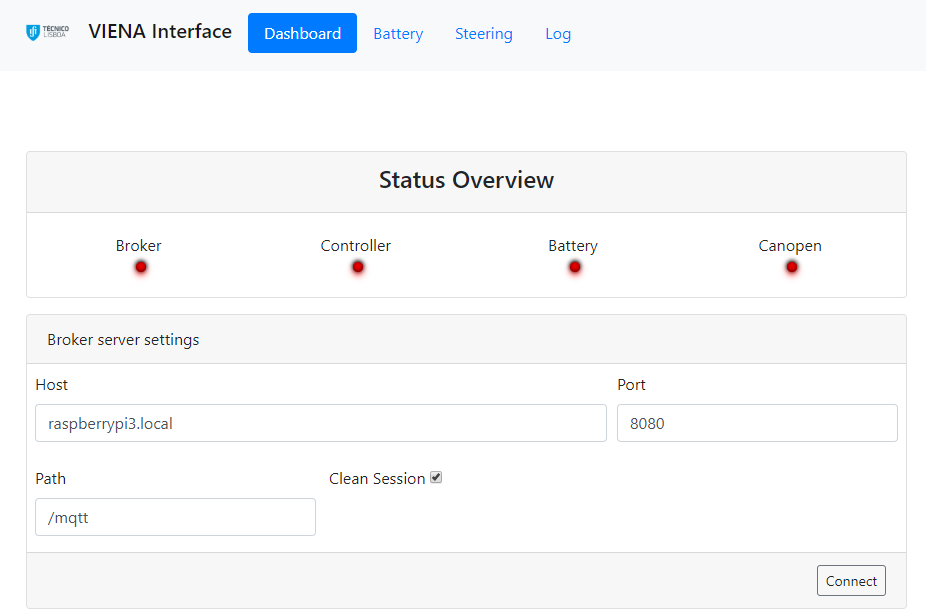
\includegraphics[width=0.7\linewidth]{figures/viena_interface}
	\caption{Current interface webpage}
	\label{fig:interface_viena}
\end{figure}

\subsection{Configure firewall}
First enable firewall by using \console{sudo ufw enable}. After use the following console command to enable the previously configured ports for ssh connection, mqtt connections and http server configured in nginx:
\begin{lstlisting}[frame=none,language=bash,backgroundcolor=\color{gray!15},numbers=none,		basicstyle=\ttfamily]
sudo ufw allow 22
sudo ufw allow 80
sudo ufw allow 1883
sudo ufw allow 8080
\end{lstlisting}
If needed, confirm status with \console{sudo ufw status}. For more advanced use run \console{man ufw}.

%-------------------------------------------------------------------------------
% create a Troubleshooting section
%-------------------------------------------------------------------------------
\section{Troubleshooting}

\begin{description}[style=nextline]
\item [The command \console{arp -a} do not show my \gls{Rpi}] In that case, try use the \console{sudo nmap -sS 192.168.1.0/24}, assuming the 192.168.1.0/24 is your local network. This is a time consuming command!
%---------------------------------------------------------------------------	
\item [Cannot find my \gls{Rpi} IP. Is it even running?] Maybe there is some problem with boot or bad microSD reading. The easiest solution is to connect a monitor and keyboard. Check messages at boot time. If nothing seems strange, manually login and then check if ehternet connection is ok using \console{ifconfig}
%---------------------------------------------------------------------------
\item [\gls{CAN} seems to not be working] First see if MCP2515 is successfully connected. 
\begin{enumerate}
\item Use \console{dmesg \textbar grep mcp2515*}. If it says successfull configured, go to next step. If not, recheck connections and restart. Also make sure the oscilator frequency match the used on boot configuration file settings as seen \hyperref[lst:boot_settings]{\textcolor{cyan}{here}}.
\item Check if can is detected as a socketcan interface. Use \console{ifconfig}. If \gls{CAN} is available, it should show a section for can0. If not, re-check if can-utils is installed.
\item View details about \gls{CAN} connection. use \console{ip -details -statistics link show can0} to get more information. If current state is \console{BUS-OFF}, manually restart the \gls{CAN} by using the following:
\begin{lstlisting}[frame=none,language=bash,backgroundcolor=\color{gray!15},numbers=none,	basicstyle=\ttfamily]
sudo ip link set can0 down
sudo ip link set can0 up \end{lstlisting}
\end{enumerate}
%---------------------------------------------------------------------------
\item[webpage is nginx default] Restart nginx service by using \console{sudo systemctl restart nginx.service}. If it still shows a different page, confirm the enabled sites are correct. Use:
\begin{lstlisting}[frame=none,language=bash,backgroundcolor=\color{gray!15},numbers=none,		basicstyle=\ttfamily]
nano /etc/nginx/sites-enabled/default
\end{lstlisting}
The default values for listen setting and root should be:
\begin{lstlisting}[frame=none,language=bash,backgroundcolor=\color{gray!15},numbers=none,		basicstyle=\ttfamily]
listen 80 default_server;
listen [::]:80 default_server;
...
root /var/www/html;

# Add index.php to the list if you are using PHP
index index.html index.htm index.nginx-debian.html;
\end{lstlisting}
If they are different, change it accordingly to meet desired configuration, by editing: \begin{lstlisting}[frame=none,language=bash,backgroundcolor=\color{gray!15},numbers=none,		basicstyle=\ttfamily]
sudo nano /etc/nginx/sites-available/default
\end{lstlisting}
If still show different then expected, try clear browser cache files.
\end{description}
